\documentclass[12pt,letterpaper]{article}
\usepackage[margin=0in]{geometry}
\usepackage{tikz}
\usepackage[T1]{fontenc}
\usepackage{lmodern}\pdfmapfile{+lm.map}
\pagestyle{empty}
\setlength{\parindent}{0pt}\hyphenpenalty=10000\exhyphenpenalty=10000
\begin{document}
\null
\begin{tikzpicture}[remember picture,overlay,x=1mm,y=-1mm]
\begin{scope}[shift={(current page.north west)}]
\node[anchor=north west,inner sep=0pt,outer sep=0pt,align=left,text width=187mm] at (15,12) {\fontsize{11}{13.86}\selectfont Week 26 / Same area, different boundaries / K--1};
\node[anchor=north west,inner sep=0pt,outer sep=0pt,align=left,text width=184mm] at (15,26) {\fontsize{13}{16.38}\selectfont Keep all tiles flat and in one piece, joined along whole sides without overlaps. Count every side with no tile beside it, including sides around holes. Turns and flips count as the same shape.};
\node[anchor=north west,inner sep=0pt,outer sep=0pt,align=left,text width=184mm] at (15,66) {\fontsize{17}{21.42}\selectfont \textbf{Problem 1:} Make every different shape you can with four tiles. Draw each shape and count its boundary sides.};
\begin{scope}[shift={(24,108)}]
\draw[step=9.5mm,black!27,line width=.3pt] (0,0) grid (38.0,38.0);
\end{scope}
\draw[black!27,line width=.3pt] (24,108) rectangle (62.0,146.0);
\node[anchor=north west,inner sep=0pt,outer sep=0pt,align=left] at (24,148) {\fontsize{12}{15.12}\selectfont \rule{13mm}{.3pt} sides};
\begin{scope}[shift={(123,108)}]
\draw[step=9.5mm,black!27,line width=.3pt] (0,0) grid (38.0,38.0);
\end{scope}
\draw[black!27,line width=.3pt] (123,108) rectangle (161.0,146.0);
\node[anchor=north west,inner sep=0pt,outer sep=0pt,align=left] at (123,148) {\fontsize{12}{15.12}\selectfont \rule{13mm}{.3pt} sides};
\begin{scope}[shift={(24,159)}]
\draw[step=9.5mm,black!27,line width=.3pt] (0,0) grid (38.0,38.0);
\end{scope}
\draw[black!27,line width=.3pt] (24,159) rectangle (62.0,197.0);
\node[anchor=north west,inner sep=0pt,outer sep=0pt,align=left] at (24,199) {\fontsize{12}{15.12}\selectfont \rule{13mm}{.3pt} sides};
\begin{scope}[shift={(123,159)}]
\draw[step=9.5mm,black!27,line width=.3pt] (0,0) grid (38.0,38.0);
\end{scope}
\draw[black!27,line width=.3pt] (123,159) rectangle (161.0,197.0);
\node[anchor=north west,inner sep=0pt,outer sep=0pt,align=left] at (123,199) {\fontsize{12}{15.12}\selectfont \rule{13mm}{.3pt} sides};
\begin{scope}[shift={(24,210)}]
\draw[step=9.5mm,black!27,line width=.3pt] (0,0) grid (38.0,38.0);
\end{scope}
\draw[black!27,line width=.3pt] (24,210) rectangle (62.0,248.0);
\node[anchor=north west,inner sep=0pt,outer sep=0pt,align=left] at (24,250) {\fontsize{12}{15.12}\selectfont \rule{13mm}{.3pt} sides};
\begin{scope}[shift={(123,210)}]
\draw[step=9.5mm,black!27,line width=.3pt] (0,0) grid (38.0,38.0);
\end{scope}
\draw[black!27,line width=.3pt] (123,210) rectangle (161.0,248.0);
\node[anchor=north west,inner sep=0pt,outer sep=0pt,align=left] at (123,250) {\fontsize{12}{15.12}\selectfont \rule{13mm}{.3pt} sides};
\node[anchor=north west,inner sep=0pt,outer sep=0pt,align=left] at (15,268) {\fontsize{9}{11.34}\selectfont Bellingham Math Circle / Week 26 / W26-K-v2};
\node[anchor=north east,inner sep=0pt,outer sep=0pt,align=left] at (199,268) {\fontsize{9}{11.34}\selectfont 1};
\end{scope}
\end{tikzpicture}
\newpage
\null
\begin{tikzpicture}[remember picture,overlay,x=1mm,y=-1mm]
\begin{scope}[shift={(current page.north west)}]
\node[anchor=north west,inner sep=0pt,outer sep=0pt,align=left,text width=187mm] at (15,12) {\fontsize{11}{13.86}\selectfont Week 26 / Same area, different boundaries / K--1};
\node[anchor=north west,inner sep=0pt,outer sep=0pt,align=left,text width=184mm] at (15,28) {\fontsize{17}{21.42}\selectfont \textbf{Problem 2:} Make a shortest-boundary shape and a longest-boundary shape with 5 tiles. Do the same with 6 tiles.};
\begin{scope}[shift={(15,77)}]
\draw[step=11mm,black!27,line width=.3pt] (0,0) grid (77,66);
\end{scope}
\draw[black!27,line width=.3pt] (15,77) rectangle (92,143);
\node[anchor=north west,inner sep=0pt,outer sep=0pt,align=left] at (15,146) {\fontsize{12}{15.12}\selectfont 5 tiles; shortest};
\node[anchor=north west,inner sep=0pt,outer sep=0pt,align=left] at (15,152) {\fontsize{12}{15.12}\selectfont \rule{13mm}{.3pt} sides};
\begin{scope}[shift={(114,77)}]
\draw[step=11mm,black!27,line width=.3pt] (0,0) grid (77,66);
\end{scope}
\draw[black!27,line width=.3pt] (114,77) rectangle (191,143);
\node[anchor=north west,inner sep=0pt,outer sep=0pt,align=left] at (114,146) {\fontsize{12}{15.12}\selectfont 5 tiles; longest};
\node[anchor=north west,inner sep=0pt,outer sep=0pt,align=left] at (114,152) {\fontsize{12}{15.12}\selectfont \rule{13mm}{.3pt} sides};
\begin{scope}[shift={(15,166)}]
\draw[step=11mm,black!27,line width=.3pt] (0,0) grid (77,66);
\end{scope}
\draw[black!27,line width=.3pt] (15,166) rectangle (92,232);
\node[anchor=north west,inner sep=0pt,outer sep=0pt,align=left] at (15,235) {\fontsize{12}{15.12}\selectfont 6 tiles; shortest};
\node[anchor=north west,inner sep=0pt,outer sep=0pt,align=left] at (15,241) {\fontsize{12}{15.12}\selectfont \rule{13mm}{.3pt} sides};
\begin{scope}[shift={(114,166)}]
\draw[step=11mm,black!27,line width=.3pt] (0,0) grid (77,66);
\end{scope}
\draw[black!27,line width=.3pt] (114,166) rectangle (191,232);
\node[anchor=north west,inner sep=0pt,outer sep=0pt,align=left] at (114,235) {\fontsize{12}{15.12}\selectfont 6 tiles; longest};
\node[anchor=north west,inner sep=0pt,outer sep=0pt,align=left] at (114,241) {\fontsize{12}{15.12}\selectfont \rule{13mm}{.3pt} sides};
\node[anchor=north west,inner sep=0pt,outer sep=0pt,align=left] at (15,268) {\fontsize{9}{11.34}\selectfont Bellingham Math Circle / Week 26 / W26-K-v2};
\node[anchor=north east,inner sep=0pt,outer sep=0pt,align=left] at (199,268) {\fontsize{9}{11.34}\selectfont 2};
\end{scope}
\end{tikzpicture}
\newpage
\null
\begin{tikzpicture}[remember picture,overlay,x=1mm,y=-1mm]
\begin{scope}[shift={(current page.north west)}]
\node[anchor=north west,inner sep=0pt,outer sep=0pt,align=left,text width=187mm] at (15,12) {\fontsize{11}{13.86}\selectfont Week 26 / Same area, different boundaries / K--1};
\node[anchor=north west,inner sep=0pt,outer sep=0pt,align=left,text width=184mm] at (15,28) {\fontsize{17}{21.42}\selectfont \textbf{Problem 3:} Make a shortest-boundary shape and a longest-boundary shape with 7 tiles. Do the same with 8 tiles.};
\begin{scope}[shift={(15,77)}]
\draw[step=10mm,black!27,line width=.3pt] (0,0) grid (80,60);
\end{scope}
\draw[black!27,line width=.3pt] (15,77) rectangle (95,137);
\node[anchor=north west,inner sep=0pt,outer sep=0pt,align=left] at (15,140) {\fontsize{12}{15.12}\selectfont 7 tiles; shortest};
\node[anchor=north west,inner sep=0pt,outer sep=0pt,align=left] at (15,146) {\fontsize{12}{15.12}\selectfont \rule{13mm}{.3pt} sides};
\begin{scope}[shift={(114,77)}]
\draw[step=10mm,black!27,line width=.3pt] (0,0) grid (80,60);
\end{scope}
\draw[black!27,line width=.3pt] (114,77) rectangle (194,137);
\node[anchor=north west,inner sep=0pt,outer sep=0pt,align=left] at (114,140) {\fontsize{12}{15.12}\selectfont 7 tiles; longest};
\node[anchor=north west,inner sep=0pt,outer sep=0pt,align=left] at (114,146) {\fontsize{12}{15.12}\selectfont \rule{13mm}{.3pt} sides};
\begin{scope}[shift={(15,166)}]
\draw[step=10mm,black!27,line width=.3pt] (0,0) grid (80,60);
\end{scope}
\draw[black!27,line width=.3pt] (15,166) rectangle (95,226);
\node[anchor=north west,inner sep=0pt,outer sep=0pt,align=left] at (15,229) {\fontsize{12}{15.12}\selectfont 8 tiles; shortest};
\node[anchor=north west,inner sep=0pt,outer sep=0pt,align=left] at (15,235) {\fontsize{12}{15.12}\selectfont \rule{13mm}{.3pt} sides};
\begin{scope}[shift={(114,166)}]
\draw[step=10mm,black!27,line width=.3pt] (0,0) grid (80,60);
\end{scope}
\draw[black!27,line width=.3pt] (114,166) rectangle (194,226);
\node[anchor=north west,inner sep=0pt,outer sep=0pt,align=left] at (114,229) {\fontsize{12}{15.12}\selectfont 8 tiles; longest};
\node[anchor=north west,inner sep=0pt,outer sep=0pt,align=left] at (114,235) {\fontsize{12}{15.12}\selectfont \rule{13mm}{.3pt} sides};
\node[anchor=north west,inner sep=0pt,outer sep=0pt,align=left] at (15,268) {\fontsize{9}{11.34}\selectfont Bellingham Math Circle / Week 26 / W26-K-v2};
\node[anchor=north east,inner sep=0pt,outer sep=0pt,align=left] at (199,268) {\fontsize{9}{11.34}\selectfont 3};
\end{scope}
\end{tikzpicture}
\newpage
\null
\begin{tikzpicture}[remember picture,overlay,x=1mm,y=-1mm]
\begin{scope}[shift={(current page.north west)}]
\node[anchor=north west,inner sep=0pt,outer sep=0pt,align=left,text width=187mm] at (15,12) {\fontsize{11}{13.86}\selectfont Week 26 / Same area, different boundaries / K--1};
\node[anchor=north west,inner sep=0pt,outer sep=0pt,align=left,text width=184mm] at (15,28) {\fontsize{17}{21.42}\selectfont \textbf{Problem 4:} Use six tiles to make shapes with 10, 12, and 14 boundary sides. Which numbers can you make in two different ways?};
\begin{scope}[shift={(22,68)}]
\draw[step=10mm,black!27,line width=.3pt] (0,0) grid (60,50);
\end{scope}
\draw[black!27,line width=.3pt] (22,68) rectangle (82,118);
\node[anchor=north west,inner sep=0pt,outer sep=0pt,align=left] at (22,121) {\fontsize{12}{15.12}\selectfont 10 sides};
\begin{scope}[shift={(121,68)}]
\draw[step=10mm,black!27,line width=.3pt] (0,0) grid (60,50);
\end{scope}
\draw[black!27,line width=.3pt] (121,68) rectangle (181,118);
\node[anchor=north west,inner sep=0pt,outer sep=0pt,align=left] at (121,121) {\fontsize{12}{15.12}\selectfont 10 sides};
\begin{scope}[shift={(22,132)}]
\draw[step=10mm,black!27,line width=.3pt] (0,0) grid (60,50);
\end{scope}
\draw[black!27,line width=.3pt] (22,132) rectangle (82,182);
\node[anchor=north west,inner sep=0pt,outer sep=0pt,align=left] at (22,185) {\fontsize{12}{15.12}\selectfont 12 sides};
\begin{scope}[shift={(121,132)}]
\draw[step=10mm,black!27,line width=.3pt] (0,0) grid (60,50);
\end{scope}
\draw[black!27,line width=.3pt] (121,132) rectangle (181,182);
\node[anchor=north west,inner sep=0pt,outer sep=0pt,align=left] at (121,185) {\fontsize{12}{15.12}\selectfont 12 sides};
\begin{scope}[shift={(22,196)}]
\draw[step=10mm,black!27,line width=.3pt] (0,0) grid (60,50);
\end{scope}
\draw[black!27,line width=.3pt] (22,196) rectangle (82,246);
\node[anchor=north west,inner sep=0pt,outer sep=0pt,align=left] at (22,249) {\fontsize{12}{15.12}\selectfont 14 sides};
\begin{scope}[shift={(121,196)}]
\draw[step=10mm,black!27,line width=.3pt] (0,0) grid (60,50);
\end{scope}
\draw[black!27,line width=.3pt] (121,196) rectangle (181,246);
\node[anchor=north west,inner sep=0pt,outer sep=0pt,align=left] at (121,249) {\fontsize{12}{15.12}\selectfont 14 sides};
\node[anchor=north west,inner sep=0pt,outer sep=0pt,align=left] at (15,268) {\fontsize{9}{11.34}\selectfont Bellingham Math Circle / Week 26 / W26-K-v2};
\node[anchor=north east,inner sep=0pt,outer sep=0pt,align=left] at (199,268) {\fontsize{9}{11.34}\selectfont 4};
\end{scope}
\end{tikzpicture}
\newpage
\null
\begin{tikzpicture}[remember picture,overlay,x=1mm,y=-1mm]
\begin{scope}[shift={(current page.north west)}]
\node[anchor=north west,inner sep=0pt,outer sep=0pt,align=left,text width=187mm] at (15,12) {\fontsize{11}{13.86}\selectfont Week 26 / Same area, different boundaries / K--1};
\node[anchor=north west,inner sep=0pt,outer sep=0pt,align=left,text width=184mm] at (15,28) {\fontsize{17}{21.42}\selectfont \textbf{Problem 5:} Which of these boundary lengths can you make with five tiles? Make each one you can, and tell your adult why the others will not work.};
\begin{scope}[shift={(26,68)}]
\draw[step=10mm,black!27,line width=.3pt] (0,0) grid (50,50);
\end{scope}
\draw[black!27,line width=.3pt] (26,68) rectangle (76,118);
\node[anchor=north west,inner sep=0pt,outer sep=0pt,align=left] at (26,121) {\fontsize{12}{15.12}\selectfont 8 sides};
\begin{scope}[shift={(125,68)}]
\draw[step=10mm,black!27,line width=.3pt] (0,0) grid (50,50);
\end{scope}
\draw[black!27,line width=.3pt] (125,68) rectangle (175,118);
\node[anchor=north west,inner sep=0pt,outer sep=0pt,align=left] at (125,121) {\fontsize{12}{15.12}\selectfont 9 sides};
\begin{scope}[shift={(26,132)}]
\draw[step=10mm,black!27,line width=.3pt] (0,0) grid (50,50);
\end{scope}
\draw[black!27,line width=.3pt] (26,132) rectangle (76,182);
\node[anchor=north west,inner sep=0pt,outer sep=0pt,align=left] at (26,185) {\fontsize{12}{15.12}\selectfont 10 sides};
\begin{scope}[shift={(125,132)}]
\draw[step=10mm,black!27,line width=.3pt] (0,0) grid (50,50);
\end{scope}
\draw[black!27,line width=.3pt] (125,132) rectangle (175,182);
\node[anchor=north west,inner sep=0pt,outer sep=0pt,align=left] at (125,185) {\fontsize{12}{15.12}\selectfont 11 sides};
\begin{scope}[shift={(26,196)}]
\draw[step=10mm,black!27,line width=.3pt] (0,0) grid (50,50);
\end{scope}
\draw[black!27,line width=.3pt] (26,196) rectangle (76,246);
\node[anchor=north west,inner sep=0pt,outer sep=0pt,align=left] at (26,249) {\fontsize{12}{15.12}\selectfont 12 sides};
\begin{scope}[shift={(125,196)}]
\draw[step=10mm,black!27,line width=.3pt] (0,0) grid (50,50);
\end{scope}
\draw[black!27,line width=.3pt] (125,196) rectangle (175,246);
\node[anchor=north west,inner sep=0pt,outer sep=0pt,align=left] at (125,249) {\fontsize{12}{15.12}\selectfont 13 sides};
\node[anchor=north west,inner sep=0pt,outer sep=0pt,align=left] at (15,268) {\fontsize{9}{11.34}\selectfont Bellingham Math Circle / Week 26 / W26-K-v2};
\node[anchor=north east,inner sep=0pt,outer sep=0pt,align=left] at (199,268) {\fontsize{9}{11.34}\selectfont 5};
\end{scope}
\end{tikzpicture}
\newpage
\null
\begin{tikzpicture}[remember picture,overlay,x=1mm,y=-1mm]
\begin{scope}[shift={(current page.north west)}]
\node[anchor=north west,inner sep=0pt,outer sep=0pt,align=left,text width=187mm] at (15,12) {\fontsize{11}{13.86}\selectfont Week 26 / Same area, different boundaries / K--1};
\node[anchor=north west,inner sep=0pt,outer sep=0pt,align=left,text width=184mm] at (15,28) {\fontsize{17}{21.42}\selectfont \textbf{Problem 6:} Move one tile in each shape and draw a result with the shortest boundary you can make. Which shapes can you make shorter?};
\filldraw[fill=black!13,draw=black,line width=.75pt] (15,77) rectangle ++(10,10);
\filldraw[fill=black!13,draw=black,line width=.75pt] (25,77) rectangle ++(10,10);
\filldraw[fill=black!13,draw=black,line width=.75pt] (35,77) rectangle ++(10,10);
\filldraw[fill=black!13,draw=black,line width=.75pt] (45,77) rectangle ++(10,10);
\filldraw[fill=black!13,draw=black,line width=.75pt] (55,77) rectangle ++(10,10);
\filldraw[fill=black!13,draw=black,line width=.75pt] (65,77) rectangle ++(10,10);
\begin{scope}[shift={(109,72)}]
\draw[step=10mm,black!27,line width=.3pt] (0,0) grid (80,50);
\end{scope}
\draw[black!27,line width=.3pt] (109,72) rectangle (189,122);
\node[anchor=north west,inner sep=0pt,outer sep=0pt,align=left] at (109,125) {\fontsize{12}{15.12}\selectfont \rule{13mm}{.3pt} sides};
\filldraw[fill=black!13,draw=black,line width=.75pt] (15,140) rectangle ++(10,10);
\filldraw[fill=black!13,draw=black,line width=.75pt] (25,140) rectangle ++(10,10);
\filldraw[fill=black!13,draw=black,line width=.75pt] (35,140) rectangle ++(10,10);
\filldraw[fill=black!13,draw=black,line width=.75pt] (45,140) rectangle ++(10,10);
\filldraw[fill=black!13,draw=black,line width=.75pt] (15,150) rectangle ++(10,10);
\filldraw[fill=black!13,draw=black,line width=.75pt] (35,150) rectangle ++(10,10);
\begin{scope}[shift={(109,135)}]
\draw[step=10mm,black!27,line width=.3pt] (0,0) grid (80,50);
\end{scope}
\draw[black!27,line width=.3pt] (109,135) rectangle (189,185);
\node[anchor=north west,inner sep=0pt,outer sep=0pt,align=left] at (109,188) {\fontsize{12}{15.12}\selectfont \rule{13mm}{.3pt} sides};
\filldraw[fill=black!13,draw=black,line width=.75pt] (15,203) rectangle ++(10,10);
\filldraw[fill=black!13,draw=black,line width=.75pt] (25,203) rectangle ++(10,10);
\filldraw[fill=black!13,draw=black,line width=.75pt] (35,203) rectangle ++(10,10);
\filldraw[fill=black!13,draw=black,line width=.75pt] (45,203) rectangle ++(10,10);
\filldraw[fill=black!13,draw=black,line width=.75pt] (15,213) rectangle ++(10,10);
\filldraw[fill=black!13,draw=black,line width=.75pt] (15,223) rectangle ++(10,10);
\begin{scope}[shift={(109,198)}]
\draw[step=10mm,black!27,line width=.3pt] (0,0) grid (80,50);
\end{scope}
\draw[black!27,line width=.3pt] (109,198) rectangle (189,248);
\node[anchor=north west,inner sep=0pt,outer sep=0pt,align=left] at (109,251) {\fontsize{12}{15.12}\selectfont \rule{13mm}{.3pt} sides};
\node[anchor=north west,inner sep=0pt,outer sep=0pt,align=left] at (15,268) {\fontsize{9}{11.34}\selectfont Bellingham Math Circle / Week 26 / W26-K-v2};
\node[anchor=north east,inner sep=0pt,outer sep=0pt,align=left] at (199,268) {\fontsize{9}{11.34}\selectfont 6};
\end{scope}
\end{tikzpicture}
\end{document}
